\subsection{Luftflöde genom väggar – drag}

När det blåser på fastigheten får det luften kring fastigheten att cirkulera och även träng in i 
byggnaden. När vinden ligger på med $\unit[3]{m/s}$, vinkelrätt mot nord- eller sydfasaden fås 
ett flöde som det i figur \ref{fig:windspeed} och trycket som då uppstår visas i figur 
\ref{fig:windpressure}. Tryckskillnaderna på de olika sidorna av husen kommer att driva 
ofrivillig ventilation vilket leder till energiförluster i form av infiltration.

\begin{figure}[hpbt]
\centering
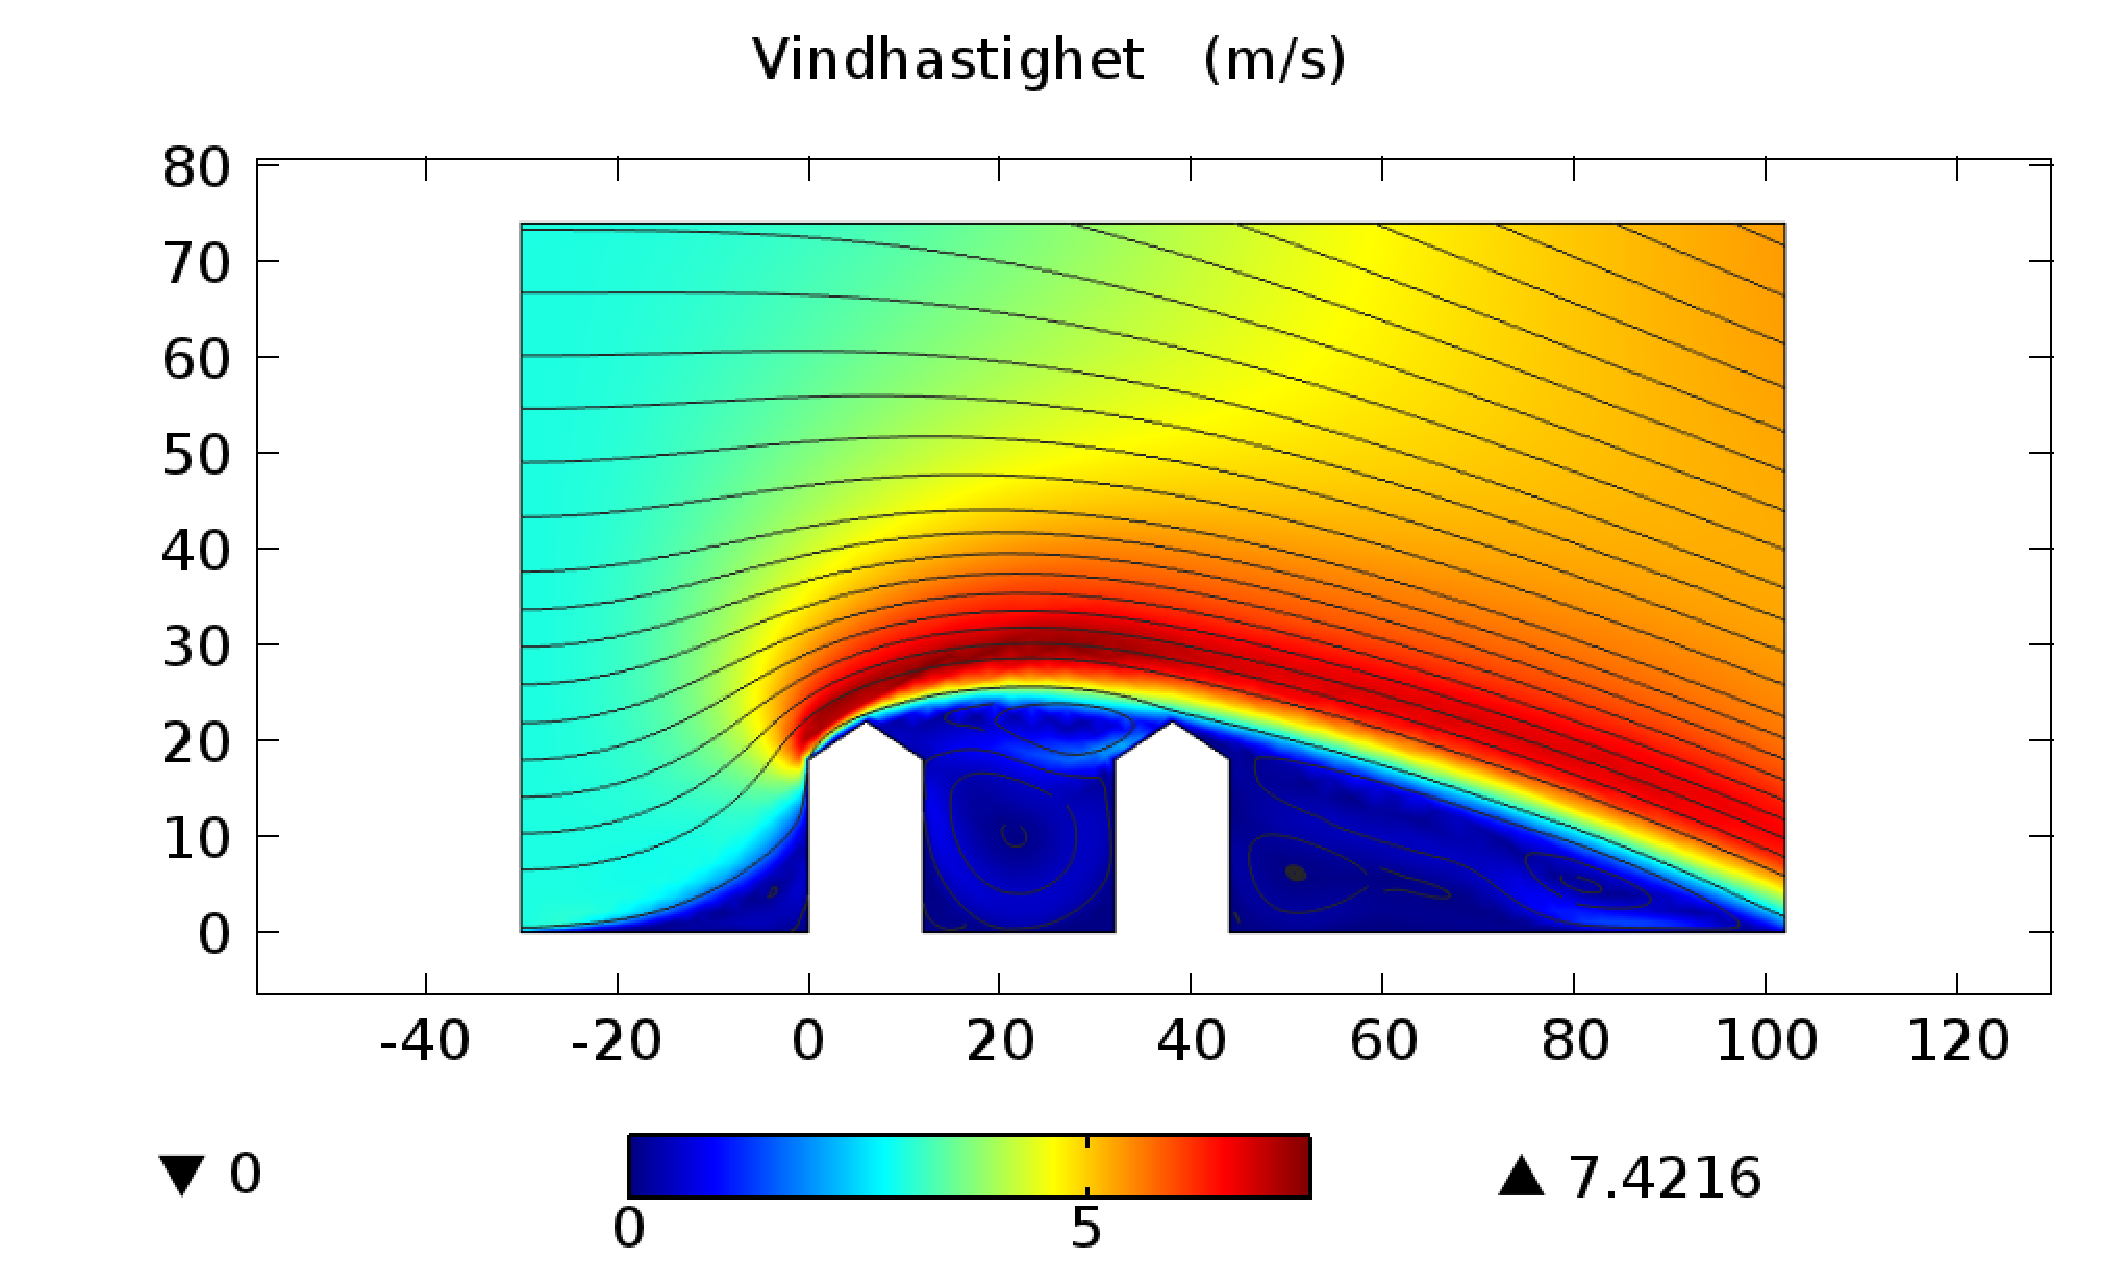
\includegraphics[width=127mm,height=76mm]{images/wind3mshdpi.eps}
\caption{\label{fig:windspeed}Vindhastiheten när vind i $\unit[3]{m/s}$ blåser mot fastigheten 
från vänster sida i figuren. Linjerna är strömlinjer och färgen indikerar farten. Värdena är 
framräknade med Comsol. Enhet m/s.}
\end{figure}


\begin{figure}[hpbt]
\centering
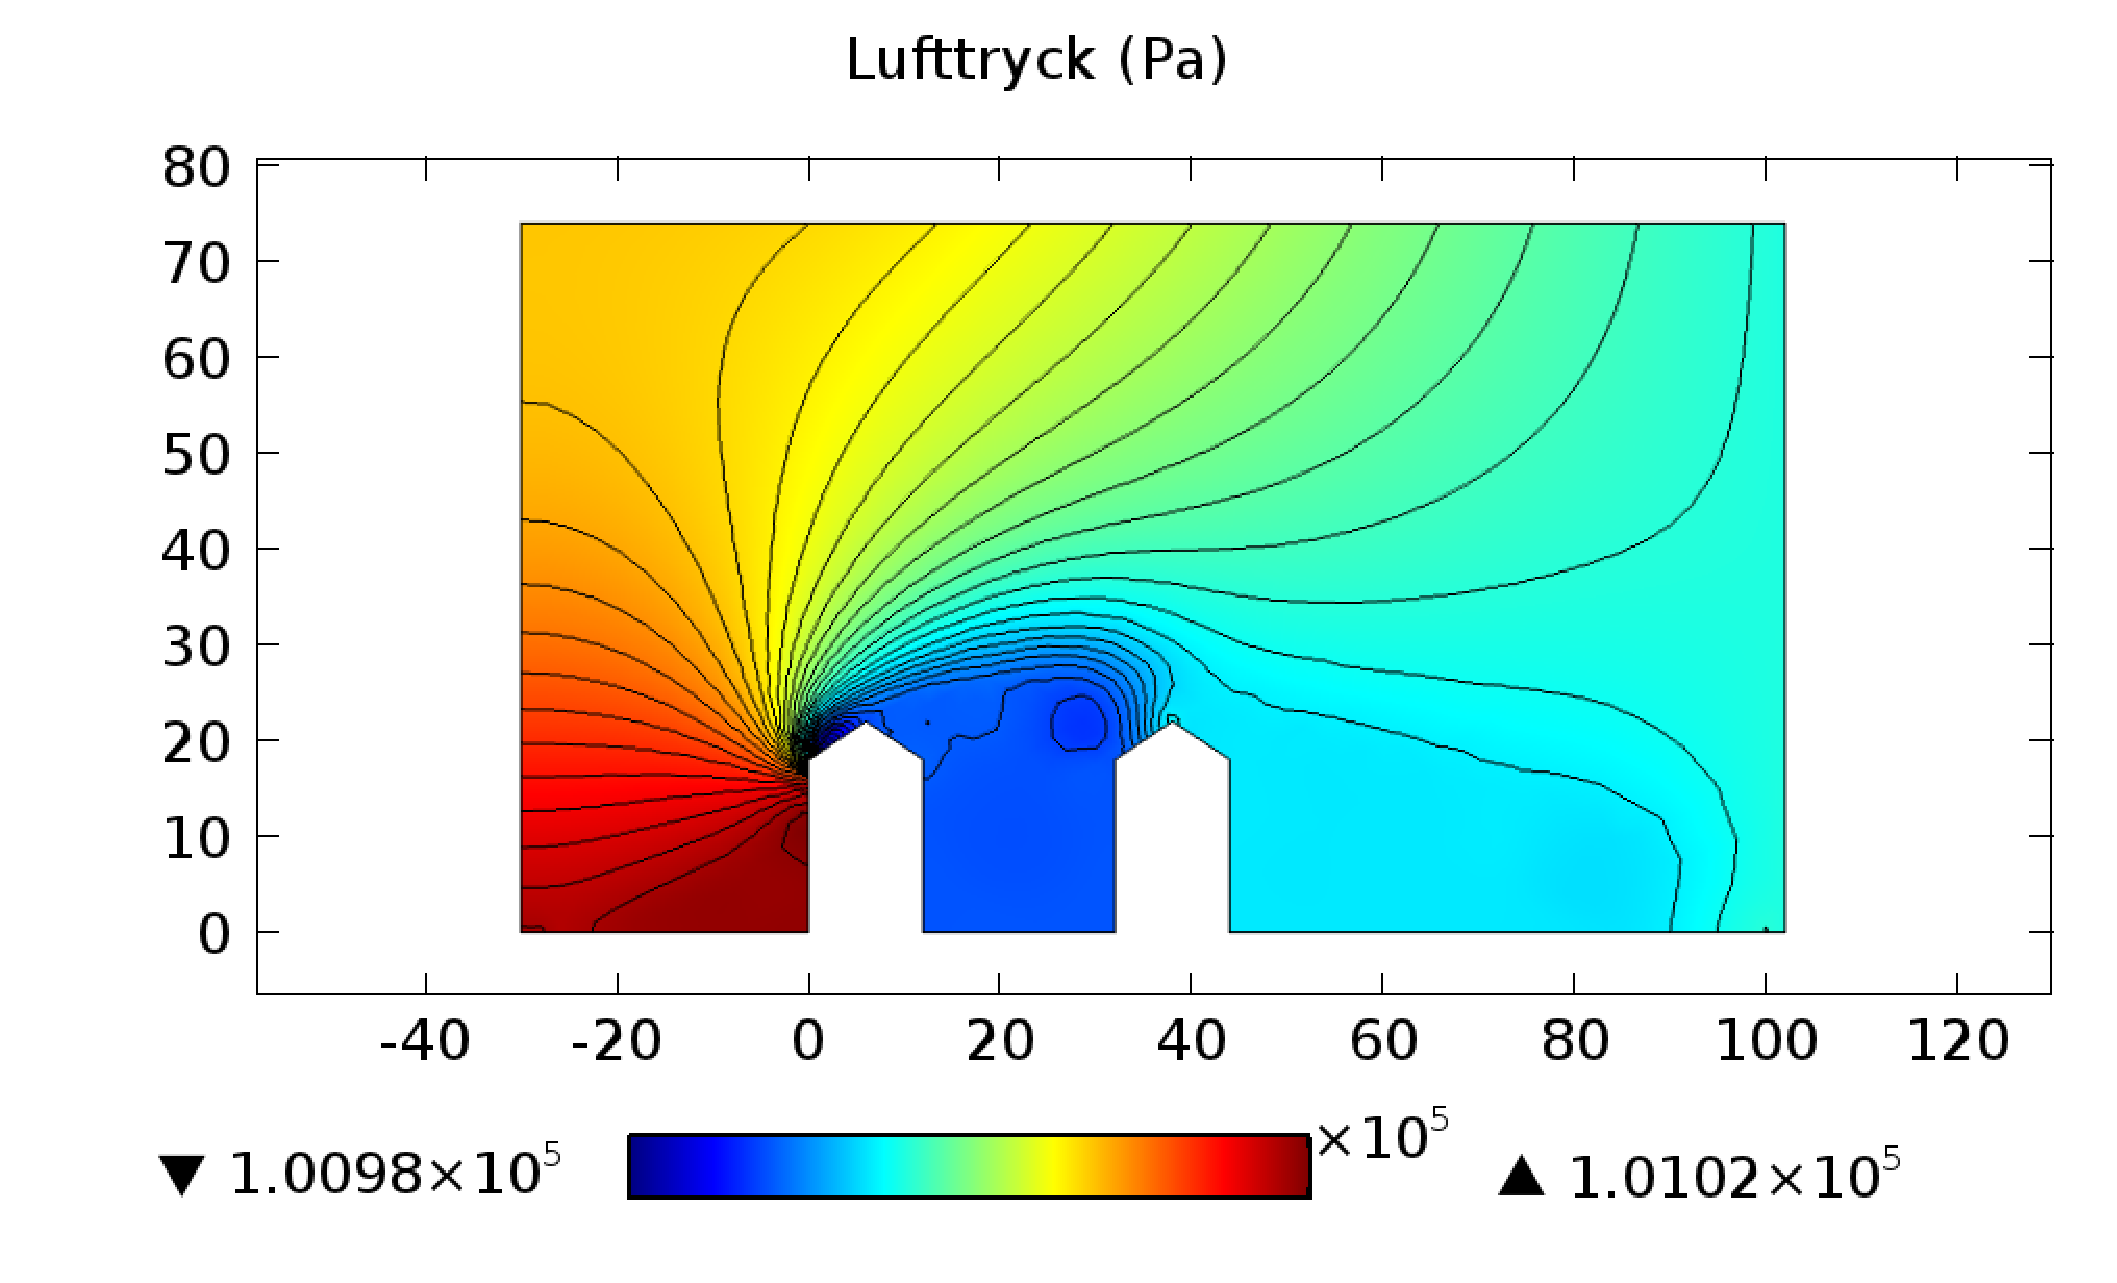
\includegraphics[width=127mm,height=76mm]{images/pressure3mshdpi.eps}

\caption{\label{fig:windpressure}Lufttrycket när vind i $\unit[3]{m/s}$ blåser mot fastigheten från vänster sida i figuren. Linjerna är isobarer, färgen indikerar lufttryck. Värdena är framräknade med Comsol. Enhet Pa.}
\end{figure}

% Resultat
Ur figur \ref{fig:windspeed} fås att det hus som ligger i lä utsätts inte för någon vind att tala om.
 Vidare fås ur figur \ref{fig:windpressure} att huset i lä utsätts för en betydligt mindre 
 tryckskillnad, än den byggnad som det blåser direkt på. I vårt exempel här, med en 
 vindhastighet runt $\unit[3]{m/s}$ fås en maximal tryckskillnad mellan norr- och sönderväggen 
 på 40 Pa, för fastigheten i lovart. Denna ökar när vindhastigheten ökar och vid 10 m/s fås en 
 tryckskillnad på 340 Pa för fastigheten i lovart. 

Applicerat på fastigheten på Walleriusgatan betyder detta att södervindar ger upphov till 
betydligt mer infiltrationsförluster än nordvindar. Till den aktuella byggnades fördel ska nämnas 
att södervindarna ofta är varmare än nordvindarna och de faktiska energiförlusterna blir 
troligen något mindre.

%%%%%%%%%%%%%%%%%%%%%%%%%%%%%%%%%%%%%%%%

Energiförlusterna på grund av drag har beräknats med ekvationerna 

\begin{equation}
Q=\frac{-kA}{\mu} \frac{(P_b - P_a)^\kappa}{L} 
\end{equation}

\begin{equation}
\Phi = AC\Delta p^\kappa;
\end{equation}

\begin{equation}
Q = \Phi\Delta T \rho c_p
\end{equation}

då är Q ett luftlöde. Vid beräkning av trycket inomhus sätts $\Phi_{in} = \Phi_{ut}$ och $C$ kan strykas om läckages är homogent fördelat över väggarna. $\kappa$ i exponenten sätts till 1 för att motsvara Darcys lag eller 0,6 vilket är ett experimentellt uppmätt värde.

\emph{\color{red} Detta är med här bara för att få ett sammanhang och förklara var de två olika kurvorna i figur \ref{fig:windenergyloss} kommer ifrån. Finns det med i något metodavsnitt jag kan hänvisa till, coh bara säga att det är en övre respektive undre uppskattning?}
 
 Energiförlusten har beräknats
  för en fastighet i lovart respektive en som ligger i lä av en annan byggnad, precis som 
  byggnaderna i figur \ref{fig:windspeed} och \ref{fig:windpressure}, vilket motsvarar att det 
  blåser på fastigheten på Walleriusgatan från söder respektive norr. Resultatet kan ses i figur 
  \ref{fig:windenergyloss} för en byggnad i lovart och en i lä samt för ett teoretiskt framtaget hus. Dessa två olika kurvor, framtagna med Darcys lag samt med det experimentella värdet på 
  0,6, får motsvara högsta respektive minsta gissningar för infiltrationsförluster i en byggnad. 

Trycken är för figur \ref{fig:windenergylossa} och \ref{fig:windenergylossb} är framräknade för 
olika vindhastigheter med programmet Comsol medan det teoretiska modellen i figur 
\ref{fig:windenergylossc} är beräknat med med en approximation. 

Approximationen baserar sig
 på att tryckskillnaden mellan inne och ute är proportionerligt med vindhastigheten i kvadrat. Denna visar hur kyleffekten blir på en rätblocksformad byggnad som ligger helt ensam. Exakta kyleffekten beror väldigt mycket på vilken omgivning byggnaden står i.


\begin{figure}[hpbt]
\centering
\subfloat[\label{fig:windenergylossa}Byggnad som vinden blåser direkt på.]{
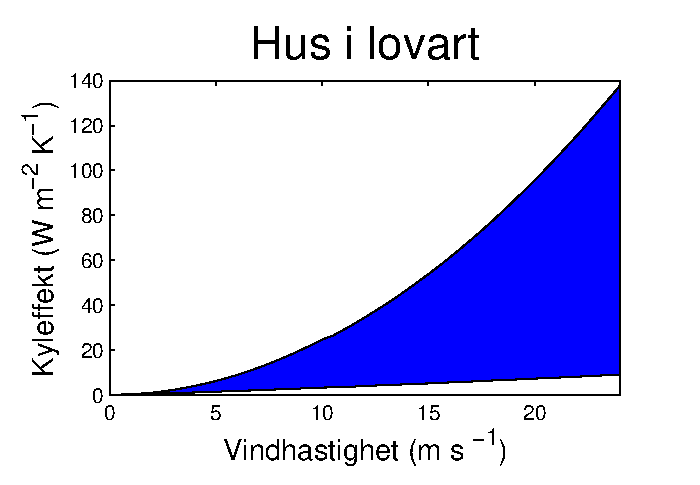
\includegraphics[width=60mm]{images/pressurewind.eps}}
\vspace{5mm}
\subfloat[\label{fig:windenergylossb}Byggnad som ligger i lä av en annan byggnad.]{
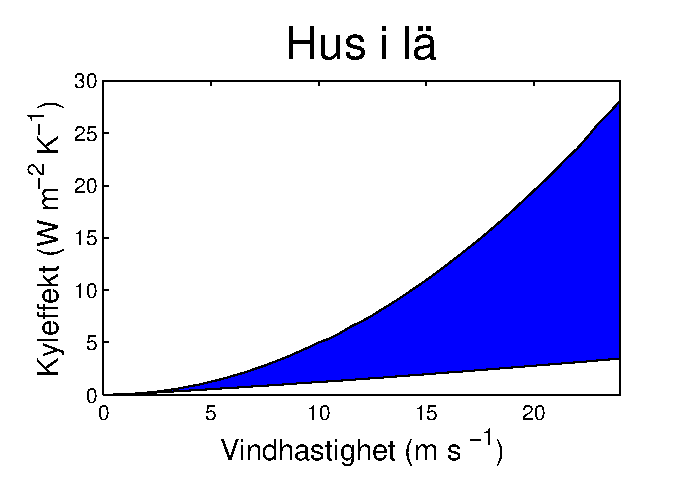
\includegraphics[width=60mm]{images/pressurenowind.eps}}

\subfloat[\label{fig:windenergylossc}Teoretisk approximation för lådformad byggnad.]{
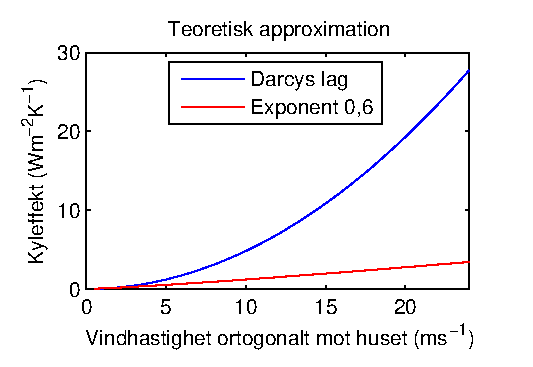
\includegraphics[width=60mm]{images/pressuretheory.eps}}

\caption{\label{fig:windenergyloss}Energiförlust per grad, max- respektive minvärde.
Framtaget med Comsol (a och b) och teoretiskt framräknade med en approximation (c).}
\end{figure}

% Resultat
Vilken kyleffekt vinden har på fastigheten är mer osäkert vid högre vindhastigheter. När vinden
 ligger på med upp emot 25 m/s kan kyleffekten variera från några tiotal watt per Kelvin upp 
 emot drygt hundra. Motsvarande kan kyleffekt för ett hus i lä vara mellan några watt per 
 Kelvin upp mot knappt trettio. För det teoretiskt beräknade huset fås även där att kyleffekten 
 kan vara mellan några watt per Kelvin upp mot knappt trettio dito. När vi har mer normala 10 
 m/s ser vi istället att kyleffekten kan vara från några få upp emot 20 W/K för en byggnad i 
 lovart, och ungefär en fjärdedel av det för en byggnad i lovart.
